\documentclass[a4paper, twoside]{article}

\usepackage{graphicx}
\usepackage{color}
\usepackage{multirow}
\usepackage{booktabs}
\usepackage[normalem]{ulem}

\usepackage{epsfig}
\usepackage{subfigure}
\usepackage{calc}
\usepackage{amssymb}
\usepackage{amstext}
\usepackage{amsmath}
\usepackage{amsthm}
\usepackage{multicol}
\usepackage{pslatex}
\usepackage{apalike}

\subfigtopskip=0pt
\subfigcapskip=0pt
\subfigbottomskip=0pt

\usepackage{siunitx}
\usepackage{multirow}
%\usepackage{tikz}

%\usetikzlibrary{calc,arrows.meta,intersections,backgrounds,shapes.misc}

\usepackage{SCITEPRESS}     % Please add other packages that you may need BEFORE the SCITEPRESS.sty package.

\begin{document}

\title{Designing an Agent for an Active Guidance System for Object Search} 

\author{
  \authorname{Anon McAnon{\sup{1}}}
  \affiliation{\sup{1}Anon University of Anon, Anonville, Anonistan}
  \email{anon.anon@anon.com}
%\affiliation{\sup{1}Lincoln Centre for Autonomous Systems (L-CAS), University of Lincoln, Lincoln, UK}
%\email{jlock@lincoln.ac.uk}
}

\keywords{Active vision, object search, vision impaired, Markov decision process}

\abstract{In this work, we propose a Markov Decision Process-based system that generates guidance instructions for a user to find a target object in an unknown environment and forms part of an active vision indoor guidance system for the visually impaired. An initial implementation of this system was implemented in an Android app and a set of experiments were carried out with sighted participants to determine its effectiveness. We found that the system works reasonably well and compares well to similar systems. }

\onecolumn \maketitle \normalsize \vfill

\section{\uppercase{Introduction}}

\noindent It is estimated that there are 440 million people worldwide that live with mild to severe visual impairments or total blindness~\cite{bourne2017magnitude} and significant effort is being made to enable these people to lead more normal and independent lives. Modern improvements to mobile computing power and image processing techniques have provided researchers with new and powerful tools to solve this problem. The ActiVis project aims to contribute to this effort by delivering an indoor navigation system targeted towards enabling blind and visually impaired (VI) users to safely navigate towards their desired destination or find an object in an unknown and dynamic environment with minimal user input. The proposed system implements ideas from the field of active vision, but replaces the electro-mechanical servo used in a typical control loop, pictured in Figure~\ref{fig:control-loop}, with a human. %This project expands upon concepts originally proposed in~\cite{bellotto2013} and~\cite{lock2017portable}.

The goal of the ActiVis system is to understand the user's surroundings and determine what the next best course of action is to reach the target location based on what is currently within view and what has been observed in the past. We trained a Markov Decision Process (MDP)~\cite{bellman1957markovian} to produce a so-called policy that defines the optimal action the agent (the guidance system in this case) takes when it finds itself within some state.  

\begin{figure}
  \centering
  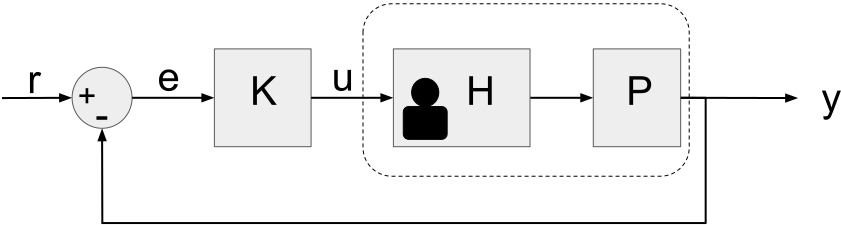
\includegraphics[width=0.45\textwidth]{figures/control_loop.png}
  \caption{The ActVis system layout and control loop. }\label{fig:control-loop}
\end{figure}

This work's contributions are 

\begin{itemize}
  \item a policy-driven human controller that can drive a user towards a point in space,
  \item a data-based MDP model that understands the spatial relationship between objects and
  \item experiments that prove the effectiveness of the system implementation.
\end{itemize}

%is the design of a guidance system and MDP (the control-block, $K$, pictured in Figure~\ref{fig:control-loop}) that can drive a user to point a mobile device's camera towards a given point in space in and find a target object. We also present and discuss preliminary experimental results to show how effective the system is at finding a target. This guidance system will be implemented into the ActiVis project upon successful tests. 

Section~\ref{sec:previous-work} discusses other relevant work done in this field, followed by a detailed discussion on the design of the ActiVis guidance system, human-control module and MDP\@ in Sections~\ref{sec:system-design} and~\ref{sec:controller-design}. Then we discuss the experiment and present its results in Section~\ref{sec:experiments}, after which we conclude the paper and discuss the project's next steps in Section~\ref{sec:conclusion}. 

\section{\uppercase{Previous Work}}\label{sec:previous-work}

\noindent Assistive vision and guidance for the VI is an active and diverse field of study. In recent years, the increase in mobile processing power and computer vision improvements have led to researchers investigating using a cellphone camera to augment or enhance a user's vision and help them find objects or another point of interest. Earlier attempts at the problem involved placing special markers or barcodes, encoded with information about an object or the area, around an environment, which the user then scans with a cellphone or similar mobile device~\cite{gude2013blind,iannizzotto2005badge3d,manduchi2012mobile}. This device then uses some feedback mode, e.g.\ Braille and sound, to guide the user towards the target. %The major drawbacks to this approach is the significant upfront effort required to augment entire areas with markers to a point where the system will be useful to a VI user. Furthermore, these passive systems rely on the user scanning the marker in the first place; something that can be made more complicated with markers degrading over time, changing ambient lighting, different viewing angles and marker occlusion. 

Another approach is to discard tags completely and rely on computer vision to perform the object detection, something that has become more plausible with recent improvements to feature detectors and deep networks~\cite{huang2017speed,redmon2016you}. The system described~\cite{schauerte2012assistive} uses a combination of SIFT and SURF to detect known objects when they are in the camera's view and guide the user to them using sonified guidance instructions. This system is more flexible than the tag-based ones, but have the same drawback of being passive and rely on chance for the user to place the object within the camera's view in the first place. The paper also does not report on any performance metrics. In~\cite{bigham2010vizwiz}, the authors discuss their VizWiz system that offloads the object recognition tasks to an Amazon Mechanical Turk worker that then provides feedback on where the object of interest is located relative to the user. The VizWiz has the advantage of being fairly robust and is able to classify a great deal of objects with little effort from the user and can provide natural, human-generated and curated directions. However, this approach does not address the issue of enhancing user independence, since the user is now beholden to an online worker instead of a relative, friend or bystander. Furthermore, a good internet connection is required on the device, perhaps limiting use in some poor-reception areas.

Researchers have begun implementing active search and perception~\cite{aloimonos2013active} strategies in robots and image classifiers in an attempt to optimise their classification and planning tasks by exploiting the structured nature of human object placements. 

In~\cite{caicedo2015active,gonzalez2015active}, the authors implemented an active search strategy for classifying objects within cluttered images. Their approaches use different methods, but both involve using a model to generate windows of interest to submit to a classifier for classification. The size and locations of the windows within the image are generated using the spatial relationship between objects, taken from the SUNCG and PASCAL datasets, and are iteratively changed based on the output from the respective models. The advantage of their approaches over their contemporaries is that far fewer windows are generated and submitted to the classifier, resulting in lower object classification times. They also report comparable accuracy when compared to their contemporaries. 

Similarly, roboticists have moved to incorporate similar strategies on robotic platforms to improve autonomous object search, manipulation and localisation tasks. The authors in~\cite{dogar2014object} developed a planning algorithm that allows a robotic manipulator to select an object to move that optimally executes an object search or exploration task in a cluttered environment. In~\cite{aydemir2011search}, the authors implemented an MDP that generates the optimal search strategy to find an object in a room over a belief state of object positions and configurations. However, the authors trained their MDP using a custom object-placement and configuration probabilities and have shown that the results are sensitive to changes within this distribution. 

In all, much research has been conducted on object recognition and guidance towards an object once detected, as well as active vision within image classifiers and robotic systems. However, work on active object search and guidance with a human is harder to come by. In this work we attempt to implement an active vision guidance system with a human in the loop~\cite{bellotto2013,lock2017portable} that can guide a user towards an out-of-view target object by using prior knowledge of the spatial distribution of objects within an indoor environment and the history of past object observations made during the search. With this, we hope to make the searching process less random and move towards a more natural and efficient object searching process to the benefit of the VI\@.  

\section{\uppercase{Active Vision System}}\label{sec:system-design}

\noindent The ActiVis project's goal is to deliver a stand-alone system that can guide a VI user to their destination with minimal user input or intervention. A complete system diagram is given is Figure~\ref{fig:control-loop}. The system design loop is similar to that of a classical control problem where a controller generates a control signal that drives a component towards some reference point. In this case, the reference signal, $r$, is the object the user wishes to find which is achieved by placing the target object within the camera's view. Therefore, the goal of the control block, $K$, is to generate guidance instructions, $u$ to drive the user along a search path towards the target object. Since we place a human in the control loop, we have an extra block, $H$, that interprets $u$ and executes a physical action, $u^*$, that manipulates the sensor, $P$, that makes a new object observation. The new observation is then fed back to the loop and the error signal, $e$, is updated accordingly.  

This work focusses on implementing $K$ and there are 2 points of interest to implementing such a controller successfully. Firstly, $K$ must be environment-agnostic, meaning that it cannot be constrained to specific environment since objects are not necessarily placed in the same place in every environment. Secondly, the controller must be robust enough to handle a badly interpreted $u$ signal. The risk of that happening can be minimised by generating clear and simple signals to help ensure that $u^*$ closely tracks $u$. 

\section{\uppercase{Human-control Module}}\label{sec:controller-design}

\noindent The guidance system is built into an Android app and uses Android's ARCore\footnote{https://developers.google.com/ar/} API to track the device's pose. The system is designed with the goal of generating a path of waypoints for the user to follow, by pointing the device camera, that will lead the user to the target object. This path is generated one waypoint at a time by the system and is updated with every object observation the user makes after adjusting the camera. We modelled and solved the search problem using an MDP model. The details of the model's design and implementation are discussed in the following sections. %For this initial design, the system only works in the pan and tilt dimension and the depth dimension will be added after successful testing of this version of the guidance system.

%\subsection{Environment Model}\label{sec:env-design}

%\noindent We model this problem on the familiar grid-world problem, where an agent is tasked move to a terminal square from an origin square given some constraints. However, instead of the traditional, linear grid-world problem, we use the grid in a radial coordinate system which surrounds the user and each grid square represent a pan/tilt angle coordinate. See Fig.~\ref{fig:environment} for an example grid. Since we do not consider the depth dimension yet, each grid square is equidistant from the user and agent. The agent translates between the squares as the user points the camera in different directions.

%\begin{figure}  
  %\centering
  %\tikzset{cross/.style={cross out, draw=black, minimum size=2*(#1-\pgflinewidth), inner sep=0pt, outer sep=0pt},cross/.default={1pt}}
\begin{tikzpicture}%[background rectangle/.style={fill=yellow!20}, show background rectangle]

  \def\thet{135}
  \def\ph{45}
  \def\l{2.2cm}
  \coordinate (O) at (0,0);
  \coordinate (U) at (3.5,-0.5);

  \node[below] (user) at ($(U)+(0,-0.4)$) {User};
  \draw[fill=black] (U) circle (0.3cm);

  \node[above] (gridlabel) at (2.3, 7.2) {Grid-world};

  % Draw the grid world outlines
  \coordinate (s0) at (0,0);
  \coordinate (s1) at (5,1);
  \coordinate (s2) at (5,6);
  \coordinate (s3) at (0,5);
  \draw[name path=bot_curve] (s0) to[out=90, in=140] (s1);
  \draw (s1) -- (s2);
  \draw[name path=top_curve] (s2) to[out=140, in=90] (s3);
  \draw (s3) -- (s0);% node[above right] {(0, 0)};

  %Draw horizontal grid lines 
  \draw[dashed] ($(s0)+(0,1)$) to[out=90, in=140] ($(s1)+(0,1)$);
  \draw[dashed] ($(s0)+(0,2)$) to[out=90, in=140] ($(s1)+(0,2)$);
  \draw[dashed] ($(s0)+(0,3)$) to[out=90, in=140] ($(s1)+(0,3)$);
  \draw[dashed] ($(s0)+(0,4)$) to[out=90, in=140] ($(s1)+(0,4)$);
  \draw[dashed] ($(s0)+(0,5)$) to[out=90, in=140] ($(s1)+(0,5)$);

  % Draw vertical grid lines
  \coordinate (v1) at ($(s0)!0.166!(s1)$);
  \coordinate (v2) at ($(s0)!0.33!(s1)$);
  \coordinate (v3) at ($(s0)!0.5!(s1)$);
  \coordinate (v4) at ($(s0)!0.66!(s1)$);
  \coordinate (v5) at ($(s0)!0.83!(s1)$);

  \draw[draw=none,name path=vert1] (v1) -- ($(v1)+(0,7)$);
  \draw[draw=none,name path=vert2] (v2) -- ($(v2)+(0,7)$);
  \draw[draw=none,name path=vert3] (v3) -- ($(v3)+(0,7)$);
  \draw[draw=none,name path=vert4] (v4) -- ($(v4)+(0,7)$);
  \draw[draw=none,name path=vert5] (v5) -- ($(v5)+(0,7)$);
  \coordinate[name intersections={of=bot_curve and vert1,by={int11}}];
  \coordinate[name intersections={of=top_curve and vert1,by={int12}}];
  \coordinate[name intersections={of=bot_curve and vert2,by={int21}}];
  \coordinate[name intersections={of=top_curve and vert2,by={int22}}];
  \coordinate[name intersections={of=bot_curve and vert3,by={int31}}];
  \coordinate[name intersections={of=top_curve and vert3,by={int32}}];
  \coordinate[name intersections={of=bot_curve and vert4,by={int41}}];
  \coordinate[name intersections={of=top_curve and vert4,by={int42}}];
  \coordinate[name intersections={of=bot_curve and vert5,by={int51}}];
  \coordinate[name intersections={of=top_curve and vert5,by={int52}}];
  \draw[dashed] (int11) -- (int12);
  \draw[dashed] (int21) -- (int22);
  \draw[dashed] (int31) -- (int32);
  \draw[dashed] (int41) -- (int42);
  \draw[dashed] (int51) -- (int52);
  
  % Draw user node and viewing angles
  \coordinate (c) at ($(U)+({\l*cos(\thet)}, {\l*sin(\thet)})$);
  \coordinate (cpan) at ($(c)+({-tan(\ph)*cos(\ph)}, {-tan(\ph)*sin(\ph)})$);
  \coordinate (ctilt) at ($(c)+({tan(\ph)*sin(\ph)}, {tan(\ph)*cos(\ph)})$);

  \draw[-Latex,] (U) -- coordinate (carc) (c) node[below] {C};
  \draw[dashed,-Latex] (U) -- coordinate (cpanarc) (cpan);
  \draw[dashed,-Latex] (U) -- coordinate (ctiltarc) (ctilt);

  \draw[-Latex] (carc) to[out=190, in=80] (cpanarc) node[right, yshift=0.13cm] {$\phi$};
  \draw[-Latex] (carc) to[out=80, in=190] (ctiltarc) node[below left] {$\theta$} ;

  % Add objects
  \coordinate (obj1) at ($(v1)!0.5!(v2) + (0,1.8)$);
  \coordinate (obj2) at ($(v3)!0.5!(v4) + (0,3.7)$);
  \coordinate (obj3) at ($(v2)!0.5!(v3) + (0,4.8)$);

  \draw (obj1) node[cross=3pt,rotate=12] {};
  \draw (obj2) node[cross=3pt,rotate=-3] {};
  \draw (obj3) node[cross=3pt,rotate=4] {};

  \node[left] (objectlabel) at (-0.4,2) {Objects};

  \draw[->] (objectlabel) -- ($(obj1)+(-0.1,0)$);
  \draw[->] (objectlabel) -- ($(obj2)+(-0.1,-0.1)$);
  \draw[->] (objectlabel) -- ($(obj3)+(-0.1,-0.1)$);

\end{tikzpicture}

%\caption{A diagram of the radial grid-world used in the MDP is modelled with. }\label{fig:environment}
%\end{figure}

%MDPs are well-suited to solving this class of problem, i.e.\ to find the optimal route from the origin square to the terminal square, so modelling our problem as a grid-world allows us to design our guidance system and MDP model with existing and well-understood models and techniques. Each square of the grid represents a combination of the agent's pan-tilt-observation, or state, which is discussed in more detail in Sec.~\ref{sec:states}. The terminal square is the square whose state contains the target object, or observation. The grid size can be adjusted to control the model's resolution: smaller squares will increase accuracy, but at the cost of performance, both during use (more squares need to be traversed) and training (much larger state space). For the initial system design, we set the grid resolution to \SI{30}{\degree}.

\subsection{MDP for Human Control}

\noindent An MDP is used to produce a policy that defines a set of optimal actions for an agent to take in any given pre-defined state. In this case, the agent is defined as the guidance system and the policy is used to generate the next waypoint on the search path towards the target object. We assume perfect state and transition observability for each timestep and the problem is given by the 5-tuple

\begin{equation}
  (\mathbf{S}, \mathbf{A}, \mathbf{T}, \text{R}, \gamma), 
\end{equation}
where $\text{R}$ is the reward function defining the immediate reward the agent receives for reaching state $s'$ after executing action $a$ in state $s$, $\mathbf{S}$ is a set of possible states the agent can be in and $\mathbf{A}$ is a set of possible actions an agent can take in any given state. $\mathbf{T}$ is a set of state transition probabilities defining the probability of transitioning from state $s$ to state $s'$ after executing action $a$ and $\gamma$ is a discount factor which prioritises immediate over long-term rewards. Each of these elements are defined and discussed next.

\subsubsection{States}\label{sec:states}

\noindent The state is a combination of parameters that defines the agent's world and decision process. The agent's state vector is given by 

\begin{equation}
  s = \langle{}o, n, v\rangle, s\in{}\mathbf{S}, 
\end{equation}
where $o$ is the current object in view, $n$ is the number of steps taken since the search started and $v$ is a binary variable that tracks whether a waypoint has been generated in the same pan/tilt position before during the search. 

\subsubsection{Actions}

The policy produced by an MDP define the action an agent will take when it finds itself in any given state. In this case, the action is the direction the next waypoint should be generated relative to the device's current view pose. The actions are defined by

\begin{equation}
  a = \langle{}s\rangle, a\in{}\mathbf{A},
\end{equation}
and the possible actions are

\begin{equation}
  \mathbf{A} = \{UP, DOWN, LEFT, RIGHT\}.
\end{equation}
%These actions were chosen to conform to the grid implementation and increase the tracking performance of $u^*$ w.r.t\@ $u$. 

Consider the scene in Figure~\ref{fig:route-example} which contains a number of simple, distinct objects (the red boxes). The MDP's task is to direct the user to point the camera to the target object (the mug in the bottom-left of Figure~\ref{fig:route-example}). It does this by inferring the current state by sampling the object currently within the camera's view, and generates an action that leads the user to the target object. The states are sampled and the actions are generated in discretised steps as the user moves the camera's view in the instructed direction. This discrete behaviour is similar to a waypoint navigation approach where the user goes from one waypoint to the next, until the user points the camera to target object. 

\begin{figure}
  \centering
  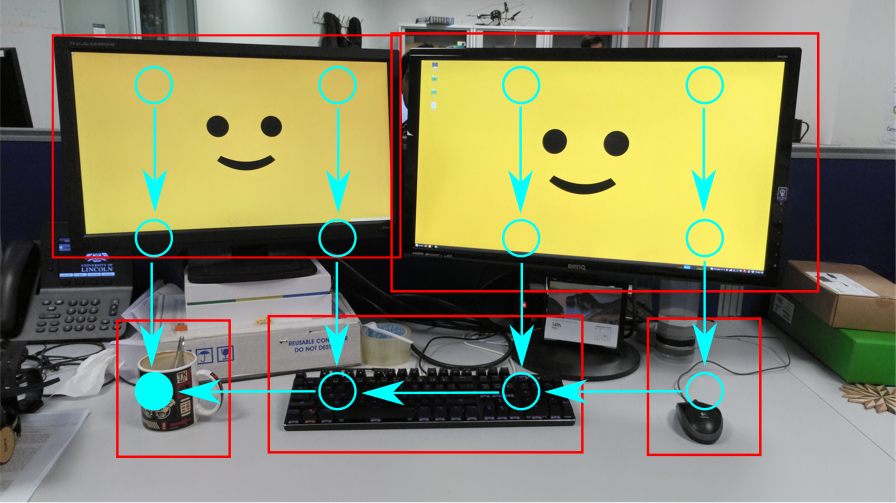
\includegraphics[width=0.5\textwidth]{figures/office_desk_example.png}
  \caption{An example of a guidance strategy the MDP generates. }\label{fig:route-example}
\end{figure}

\subsubsection{State Transition Probabilities}

\noindent The state transition function, $\mathbf{T}$, defines the probability of the agent transitioning into state $s'$ from state $s$ when taking action $a$, i.e.\ the likelihood of moving to a new pan/tilt position and observing object $o$ after performing action $a$. Therefore, $\mathbf{T}$ represents the spatial relationships between the different objects in the environment model. Formally, the transition function is defined by

\begin{equation}
  t=\langle{}s, a, s'\rangle, t\in{}\mathbf{T}.
\end{equation}

\subsubsection{Reward Function}

\noindent The reward function, $R$, is the immediate reward that the agent receives after transitioning from state $s$ to state $s'$ and is given by 

\begin{equation}
  R = r(s, s').
\end{equation} 

The goal of the agent is to maximise the cumulative reward it receives and is a very important parameter for producing a good policy that will define the optimal action for the agent to execute for any given state. In order to encourage the agent to actively search for the target object, a set of negative rewards must be defined, along with a relatively large positive reward for successfully reaching the target object. These parameters must be finely balanced to ensure efficient object search behaviour from the agent.

%The reward function is a very important parameter for training the agent to produce the most effective policy. We define a constant negative reward for every step the agent takes, and increase this negative reward if the agent exceeds the 12-step limit we defined in the model, as well as if it regenerates a waypoint in a previously searched location. The values we used were empirically chosen and are given in Table~\ref{tab:rewards}.

%The goal of the agent is to maximise its cumulative reward over time and these numbers are chosen such that they actively motivate the agent to reach the target, while hastening the process by slightly punishing it for each step it takes and increasing the punishment every time it re-explores a state and the longer it takes to reach the target. 

\subsection{MDP Implementation}

\subsubsection{Model Training}

\noindent A policy that defines the optimal action for an agent to take for any given state is generated through a training process that involves letting the agent explore the entire state-space and iteratively improve its decision function, i.e.\ policy, in order to reach the target state in a way that maximises its cumulative reward. This method is called Q-learning and does not require a model of its environment during training. 

The agent's target state is any state where $s = \langle{}o=o_{target}, n, v\rangle$. This gives a total of 14 terminal states (7$\times$2) per policy, since the target object can can be found at any point in the search or in a position that was previously explored by the agent and user. Each target object has its own unique policy file.

The reward function was crafted by hand and the parameters were empirically selected. The function values can be found in Table~\ref{tab:rewards}. $R$ punishes the agent for every step it takes where it does not find the target object and the negative reward is increased if the agent is taking too long to find the target ($n > n_{\max}$) or when it generates a waypoint in a location that it has generated a waypoint previously ($v = true$). Conversely, it gives a significant positive reward when the target object is found. 

\begin{table}
  \centering
  \caption{The reward functions for the MDP.\ }\label{tab:rewards}
  \begin{tabular}{ll}
    \toprule
    $r(s, s'), s\in\mathbf{S}$ & -1  \\ \midrule
    $r(n > n_{\max})$ & -10 \\ \midrule
    $r(v = true)$  & -10 \\ \midrule
    $r(o = o_{target})$ & 10000 \\ \midrule
    \bottomrule
  \end{tabular}
\end{table}

Currently there are 8 objects encoded into the system, including a `nothing' instance where nothing of note is observed. Our initial implementation considers a simple office desk scenario containing the following objects:

\begin{equation}
  \begin{aligned}
    o\in \mathbf{O} = \{monitor, mouse, keyboard, window,\\mug, stationary, desk, nothing\}.
  \end{aligned}
\end{equation}

The spatial relationships between the objects in $\mathbf{O}$ are extracted from the OpenImage dataset\footnote{https://storage.googleapis.com/openimages/web/index.html}~\cite{openimages} that consists of 1.74M images containing 14.6M manually drawn and labelled bounding boxes around objects (see Figure~\ref{fig:openimage-example} for an example) and is primarily aimed toward object recognition researchers to benchmark their models. The bounding boxes and object labels are used to extract the spatial relationships between the different objects in $\mathbf{O}$. Since the camera perspectives and absolute distances between the objects in the images are not given, we can only extract the relationships in the basic action terms specified in $\mathbf{A}$, e.g.\ we can only say that object 1 is above object 2, but not how far above. Our simple action-space and grid environment somewhat compensates for the dataset's lack of complexity. 

\begin{figure}
  \centering
  \begin{subfigure}
    \centering
    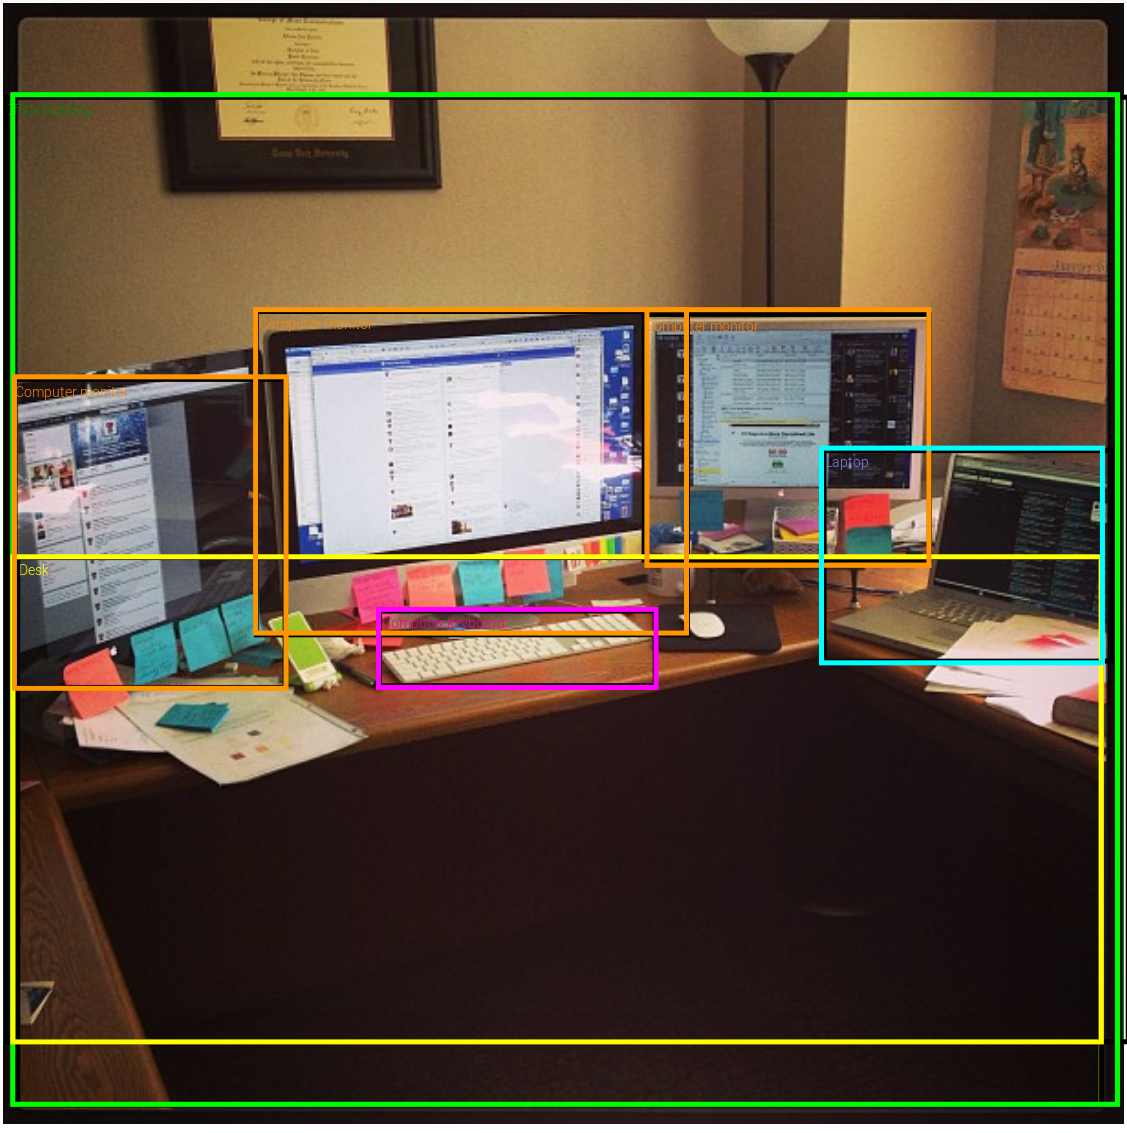
\includegraphics[width=0.4\textwidth]{figures/desk_example.png}
  \end{subfigure}
  \begin{subfigure}
    \centering
    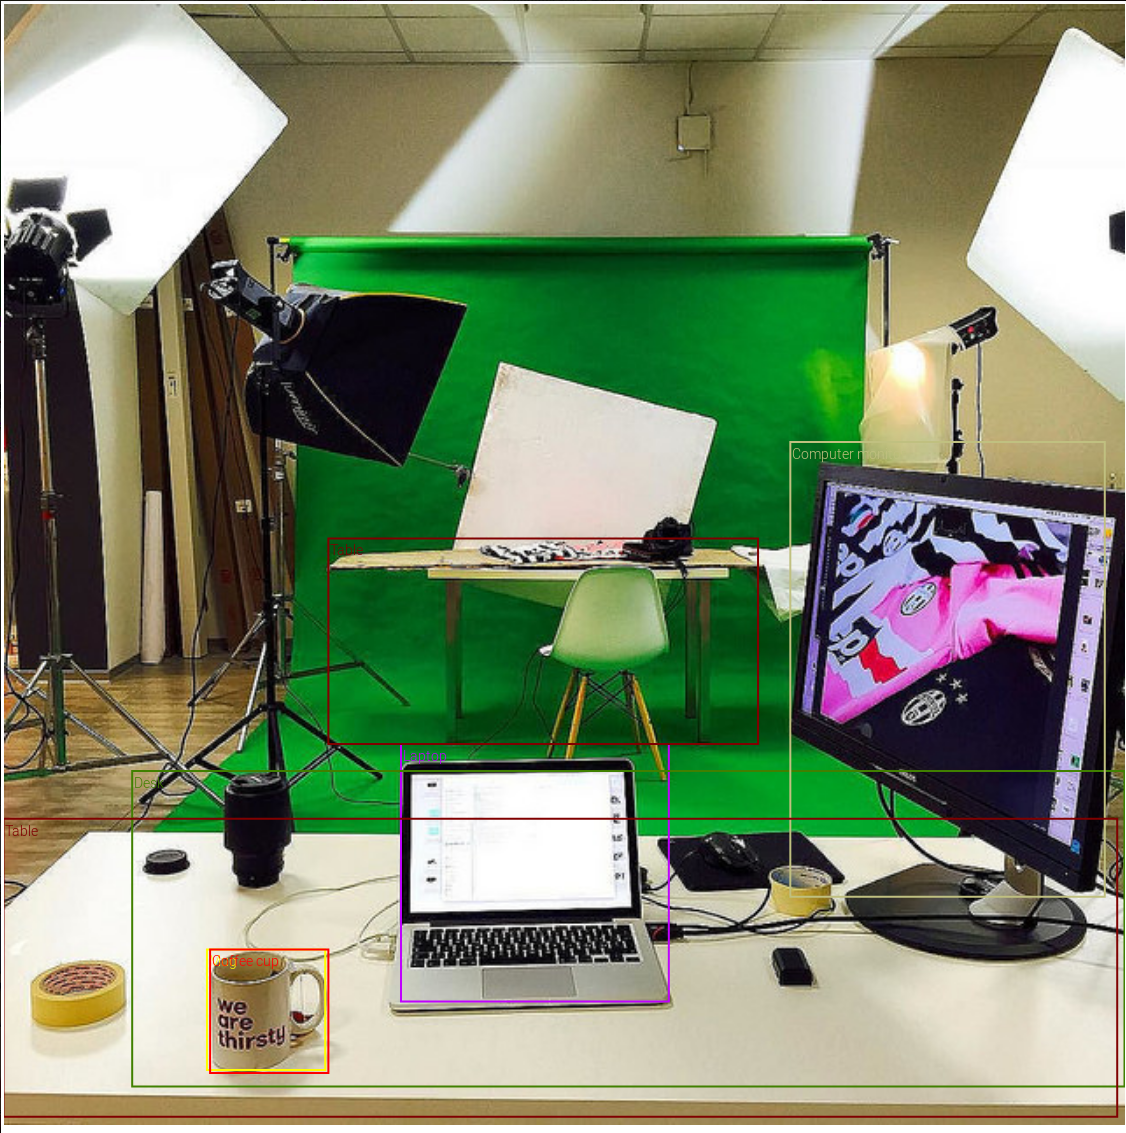
\includegraphics[width=0.4\textwidth]{figures/mug_example.png}
  \end{subfigure}
  \caption{Examples of images from the OpenImage dataset containing objects from $\mathit{O}$~\cite{openimages}. }\label{fig:openimage-example}
\end{figure}

Figure~\ref{fig:obj-relationships} shows the spatial relationship between a subset of $\mathbf{O}$ (desk, keyboard and mouse). For example, when the agent is in state $s=\langle{}o=mouse, n, v\rangle$ and searching for a keyboard, there is a strong probability that the target object is $LEFT$ of the mouse. The MDP model considers all of the objects' spatial relationships when generating the optimal policy.

\begin{figure}
  \centering
  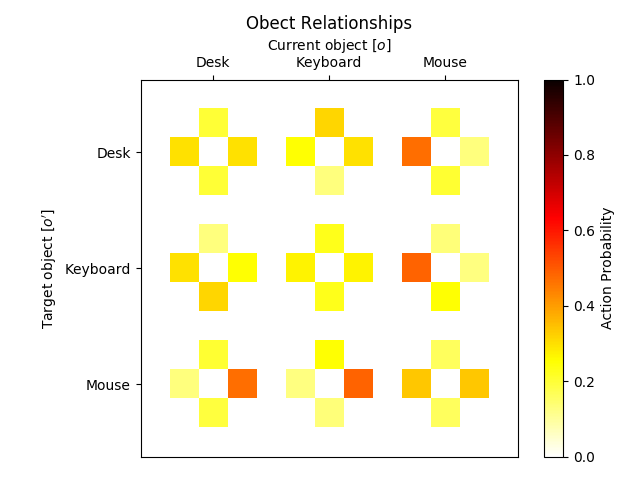
\includegraphics[width=0.5\textwidth]{figures/object_relationships.png}
  \caption{Examples of the spatial relationships between the desk, keyboard and mouse objects. Each square corresponds to the probability of executing the action that square represent (top square for $UP$, etc.)}\label{fig:obj-relationships}
\end{figure}

We set the model to track a maximum of of 11 (inclusive) steps to the target, with 11 being the longest possible route on the grid (more details about the grid are in Section~\ref{sec:system-implementation}). A search can take longer than 11 steps, but the MDP considers anything greater than 9 steps as the maximum, which is convenient for keeping a manageable state-space and a simple reward function. The MDP therefore has a total of 154 reachable states ($s_{total}=11\times7\times2$).

The lack of absolute spatial information in the OpenImage dataset generates ambiguities which makes it hard for the model to converge to a single, optimal solution. We therefore could not use the popular value iteration algorithm~\cite{bellman1957markovian} and opted for the state-action-reward-state-action (SARSA) algorithm~\cite{rummery1994line} instead. SARSA is an on-policy algorithm that allows us to control the level of exploration vs.\ exploitation that makes it easier to find a solution, but this solution is not guaranteed to be optimal. 

The model is trained until it converges to the optimal policy, or for a total of approximately 17 million episodes. The parameter, $\alpha$, that controls the exploration vs.\ exploitation behaviour during training maximises exploration when it is set to $1.0$ and exploitation when it is $0.0$. We set $\alpha$ to a function that starts at a high exploration value and exponentially changes it behaviour to exploitation as it becomes more trained. $\alpha$ is given by 

\begin{equation}
  \alpha = \exp\Big(\frac{-i}{10n_{states}}\Big) - 0.001,
\end{equation}
where $i$ is the episode index.  $\gamma$ is set to 0.95 to prioritise long-term reward. 

Our MDP has a relatively small state-action space. Therefore, a solution can be found in a reasonable amount of time. However, it should be noted that adjusting the angle interval, or adding more actions or objects, can easily blow up the size of the state-space. 

\subsubsection{Android Implementation}\label{sec:system-implementation}

We incorporated the trained MDP model and policies into an Android app (see Figure~\ref{fig:system-screenshot} for a screenshot). This app is responsible for generating the guidance instructions and tracking the agent and sensor ($K$ and $P$ blocks in Figure~\ref{fig:control-loop}) throughout a search session. Tracking the agent's pose allows the app to infer the current state and look up the optimal action to take. 

\begin{figure}
  \centering
  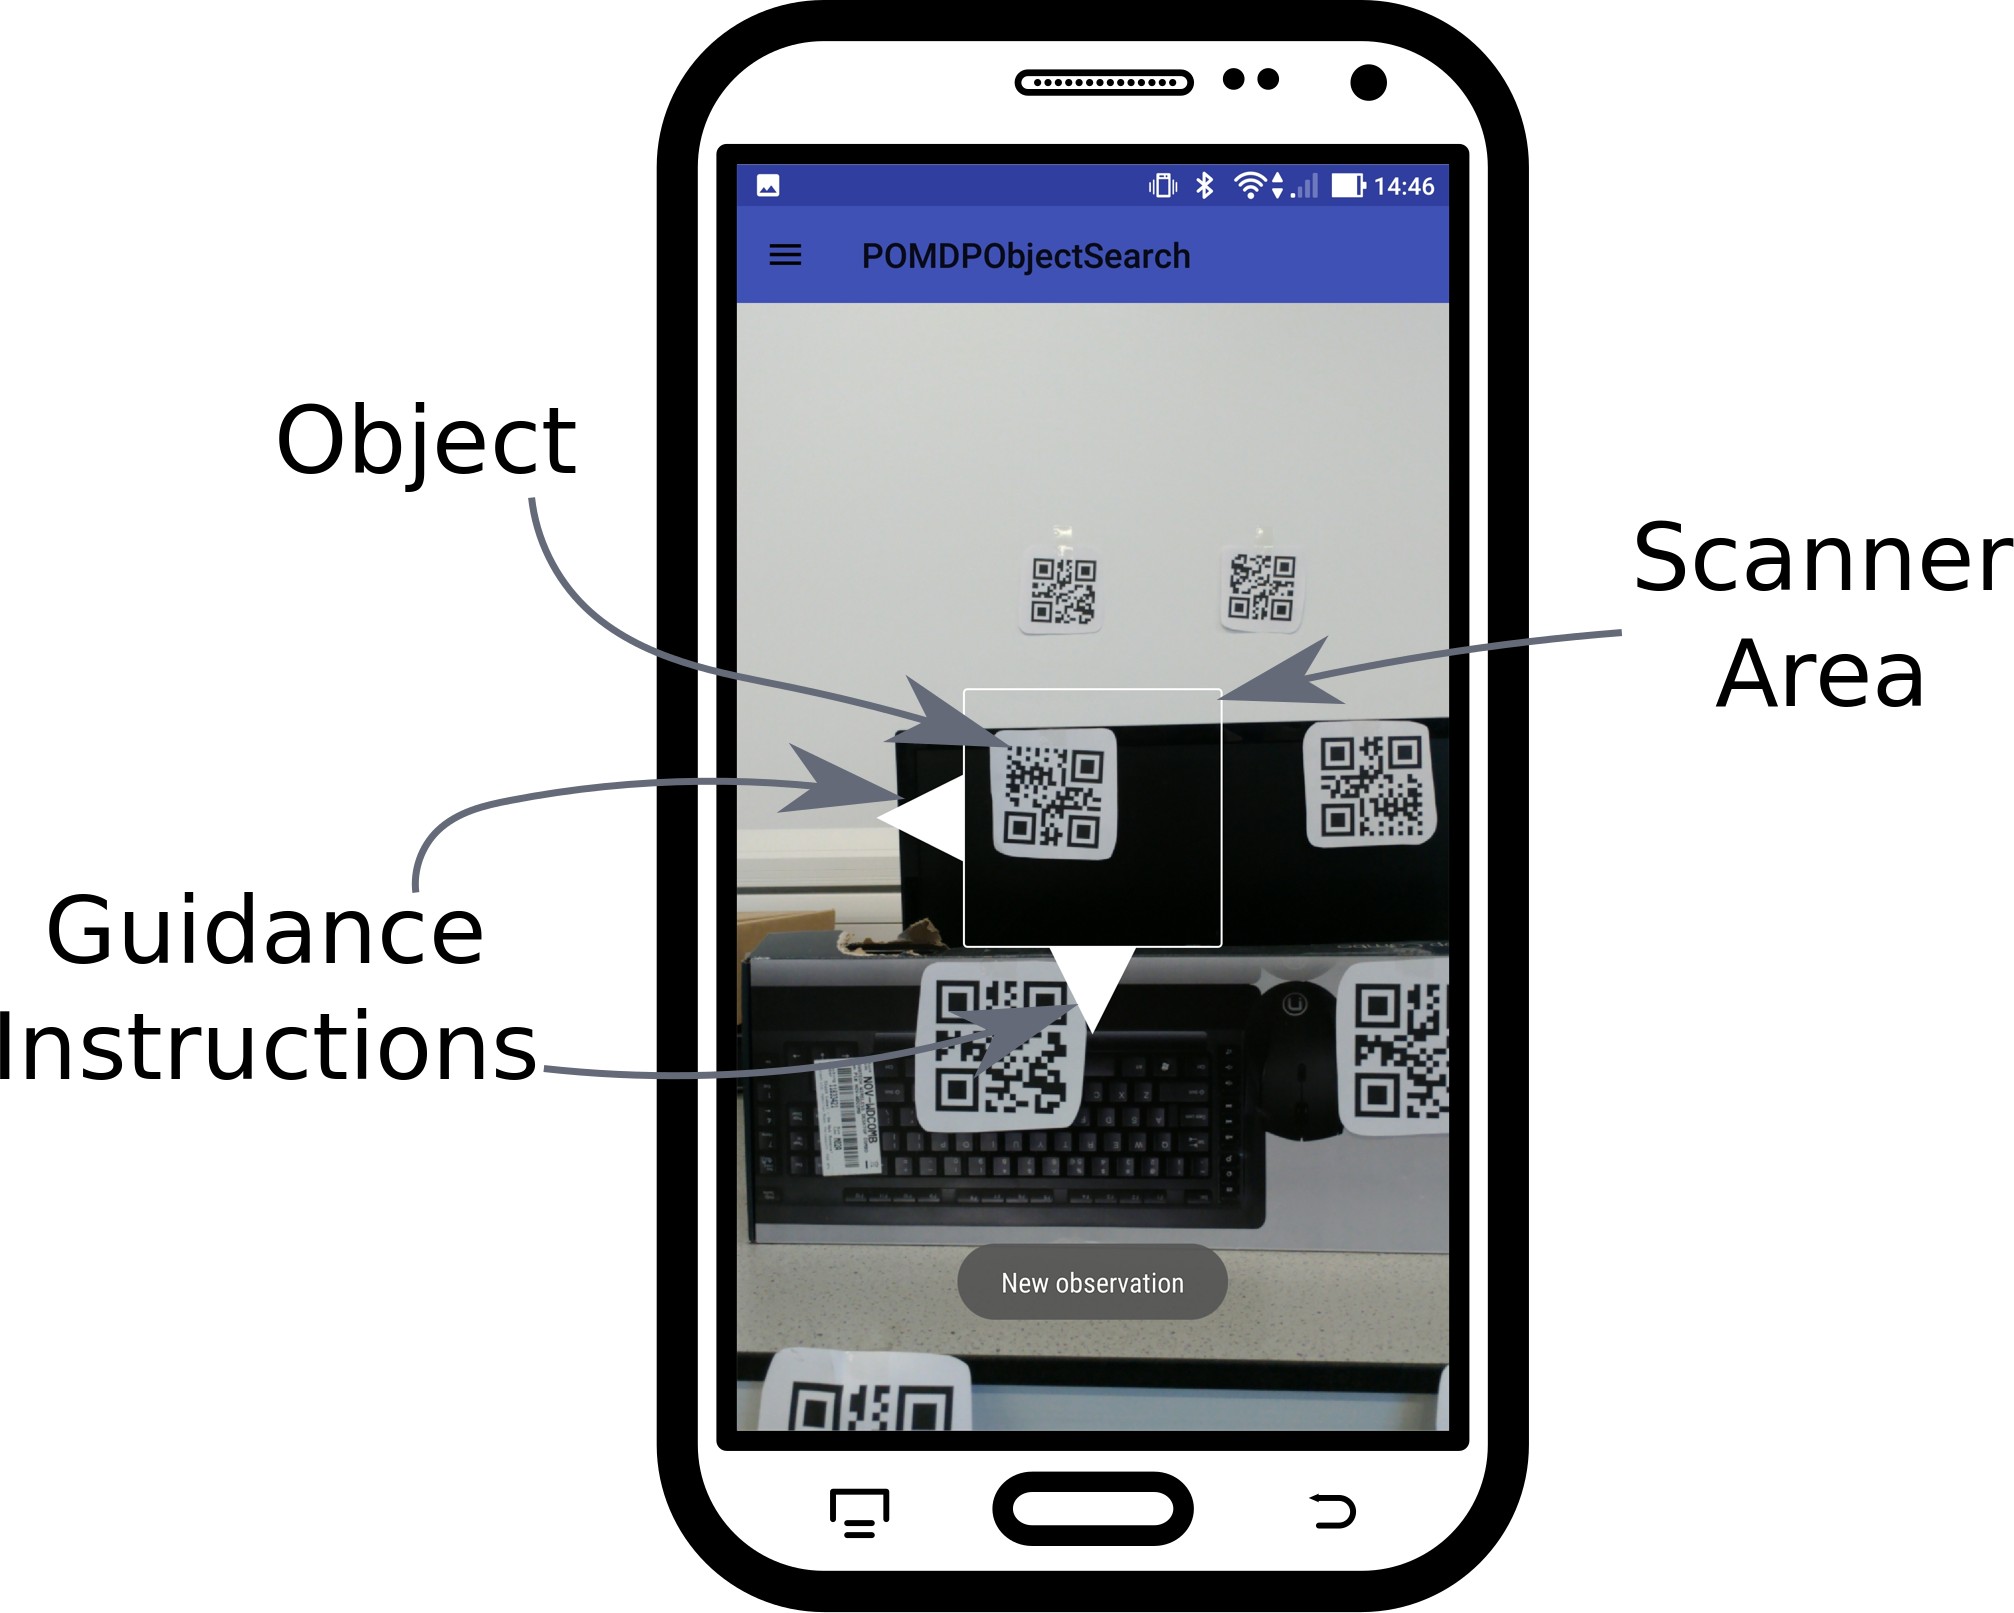
\includegraphics[width=0.45\textwidth]{figures/system_screenshot2.png}
  \caption{A screenshot of the guidance interface showing a waypoint (based on an 3D Android model), the object scanner area and the guidance instruction arrows. }\label{fig:system-screenshot}
\end{figure}

The app uses a 6$\times$6 discretised and wrapped radial grid to simplify the tracking and waypoint generation processes. In this setup, the policy action is interpreted by the app and a new search waypoint is generated in the centre of the cell specified by the action, e.g.\ an `$UP$' action will generate a waypoint one grid cell up from where the user is currently pointing the camera. The app's guidance system then uses the new waypoint's location to provide the user with guidance instructions. The grid is generated at the app's start-up and remains constant throughout the app's lifetime. The policy actions, and waypoints by extension, are given in relative to the user's current viewing pan/tilt position. The grid spans \SI{120}{\degree} in both the pan and tilt dimensions, giving a resolution of \SI{20}{\degree} per grid cell. 

By recording the previous positions and waypoint locations the app generated, it can infer the state values for $v$ and $n$. Furthermore, the camera provides the ID of the object in view, populating $o$ in the state. A real-time object detector was not used in this system to avoid unnecessary complexity and processing overhead and encoded QR codes and barcode scanner library were used to simulate object detection instead. 

The QR code scanner requires raw image data. To avoid scanning multiple QR codes and using excess processing power by scanning large images, we only used the centre part of the screen to scan for a barcode. This scanner area is $300\times300$ pixels and scans for barcodes without causing any frame-rate drops.  

The app was developed on and experimented with an Asus ZenPhone AR\footnote{asus.com/uk/Phone/ZenFone-AR-ZS571KL/} running Android version 7.0 with the ARCore SDK enabled. No hardware or software modifications were required.

\section{\uppercase{Experiments}}\label{sec:experiments}

\noindent To test the effectiveness of our MDP and its policies, we designed a set of experiments that determined how effective the system is at directing a participant to point the device's camera towards a target object. This section discusses the experiments and their results. 

\subsection{Experiment Design}

\noindent For the experiment, the MDP policies were integrated into an Android application that uses the camera to provide observation data and track the pose and viewing direction. We avoided adding unnecessary variability and complexity to the experiment by providing visual waypoints on screen which the participants were allowed to use. A generic environment mimicking a typical office desk layout was set up as the experiment environment and contains 7 different objects (i.e.\ encoded QR codes), one of which could be selected for each experiment run. See Figure~\ref{fig:env-picture} for a picture of the environment. 

\begin{figure}
  \centering
  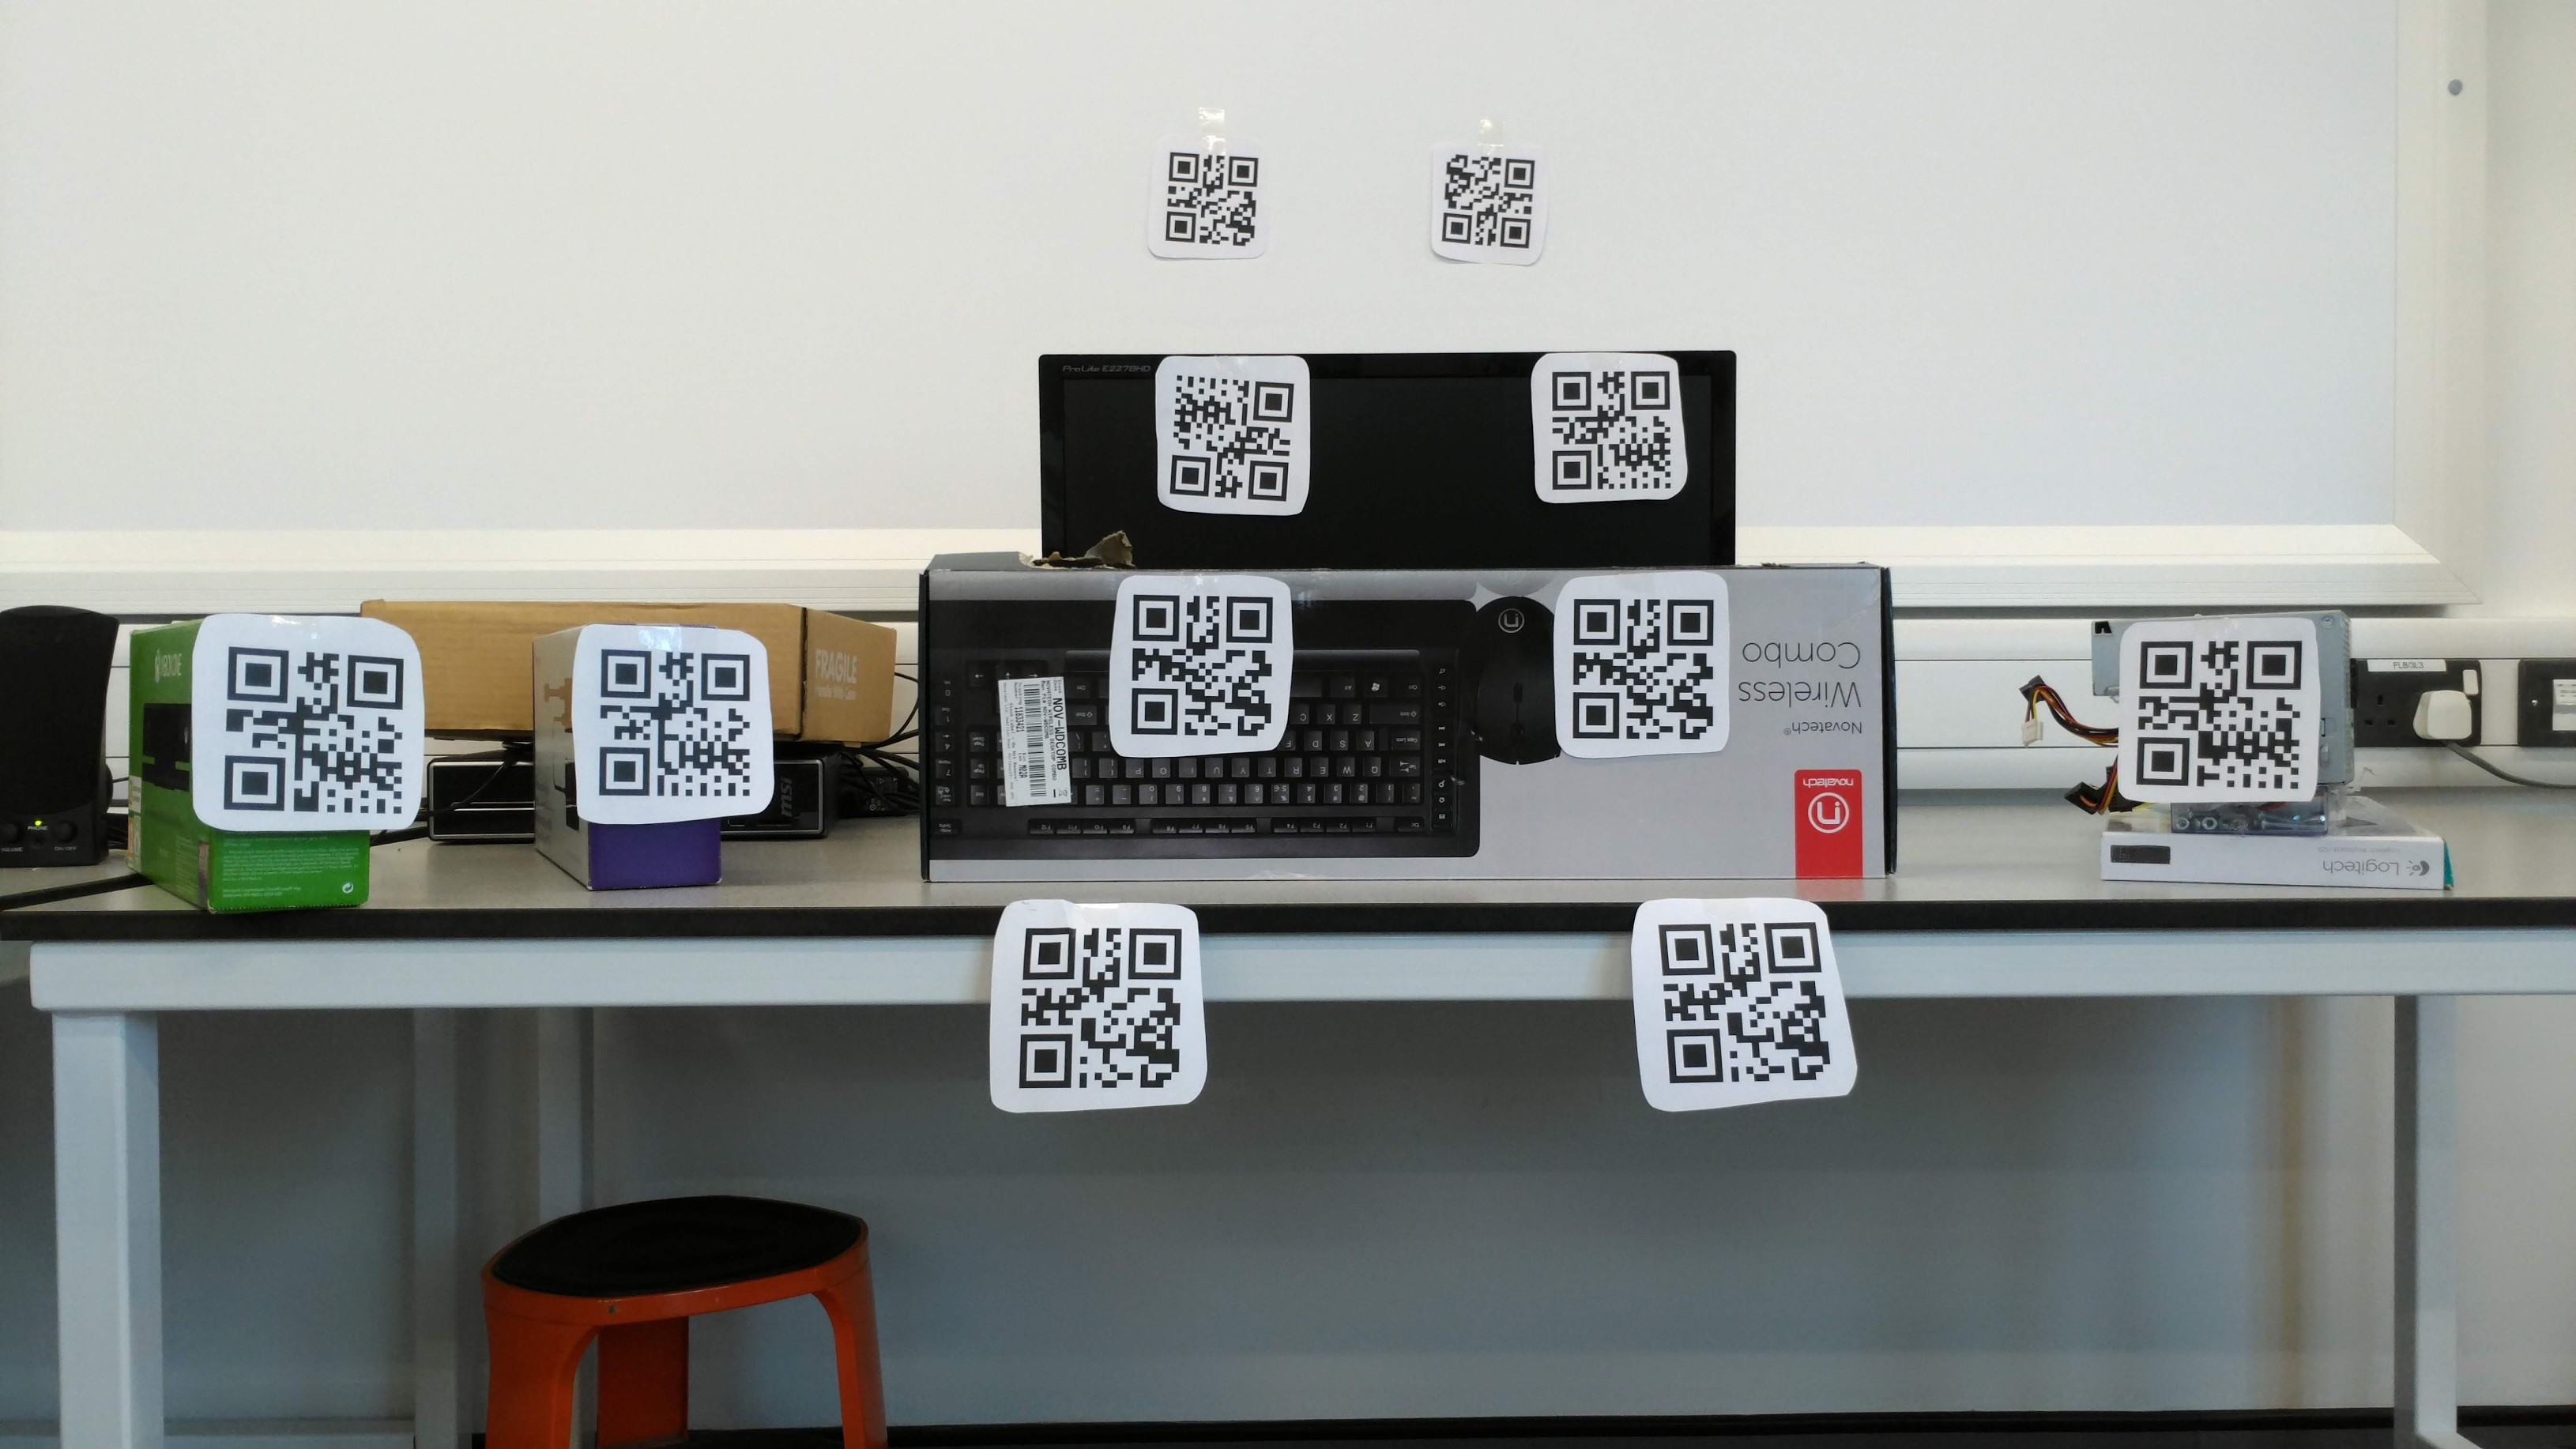
\includegraphics[width=0.4\textwidth]{figures/test_env_picture.jpg}
  \caption{A picture of the environment used for the experiments. Each QR code represents an object.}\label{fig:env-picture}
\end{figure}

For each experiment, the participant was placed roughly \SI{1}{\meter} from the barcodes and was asked not to move from that spot during the experiment. The participant then pressed a button on the app that randomly selected a target object and was then guided towards that target by the app. Since the participants were allowed to use their vision, the targets were randomly selected and the participants were uninformed of what the target object was until it was found. This was done to avoid the participants learning the target objects' locations between each search run.

During in-house tests, we noted that the system sometimes makes guidance mistakes that lead the user towards an uncluttered edge of the search space, at which point the system had difficulty guiding the user back to the centre. To avoid this having an adverse impact and drawing out the experiments too long, we set a search step limit of 15, which means that the search was terminated when the number of waypoints exceeded 15. A search run therefore ended when the participant either successfully found the target object by pointing the phone camera to it and scanning the barcode, or exceeded the waypoint limit. After this, the participant then resets to the central position, selects a new target object and resumes the experiment.

The participants were left to repeat this process until we recorded 10 searches per object, giving us a total number of 70 recorded search samples per participant. We tested a total of 10 different participants (sex: 8 M, 2 F;\@ age: $\mu$ 31.2 years, $\sigma$ 8 years), most of which were sourced from our laboratory with none having any disabilities or handicaps. This gives our dataset a total of 700 search samples.

\subsection{Results}

\noindent In order to evaluate our system, we identified 3 different measures: target acquisition rate (TAR), number of steps to the target and the total time it took to find a target object. We present and discuss the results for each of these parameters in the next sections. The results for each individual participant is presented in Table~\ref{tab:results-full} and Table~\ref{tab:results-summary} gives the results across all of the participants. 

To provide a baseline measure for the ideal case, we ran a number of simulations in an environment mimicking the experiment setup with an agent that perfectly executes the policy, i.e.\ $u=u^*$. The TAR and steps to target results for the simulation are included in Table~\ref{tab:results-summary}.

\begin{table}
  \centering
  \caption{A table containing the results for the TAR, number of steps and time to target means ($\mu$) and standard deviations ($\sigma$) for each individual participant.}\label{tab:results-full}
  \begin{tabular}{cccc}
    \toprule
    Participant & TAR [\%] & Num. Steps & Time [s] \\ \midrule
    %\multirow{2}{*}{Participant} & \multirow{2}{*}{TAR [\%]} & \multicolumn{2}{c|}{Num. Steps} & \multicolumn{2}{c}{Time [s]} \\ 
				 %&			     & $\mu$ & $\sigma$		       & $\mu$ & $\sigma$  \\ \midrule
    s1 & 94 & 7.2 $\pm$ 5.4 & 29 $\pm$ 22 \\ \midrule
    s2 & 79 & 6.7 $\pm$ 4.8 & 34 $\pm$ 5.1 \\ \midrule
    s3 & 91 & 6.3 $\pm$ 4.9 & 31 $\pm$ 21 \\ \midrule
    s4 & 79 & 6.7 $\pm$ 4.3 & 37 $\pm$ 5.6 \\ \midrule
    s5 & 76 & 7.2 $\pm$ 4.9 & 33 $\pm$ 14 \\ \midrule
    s6 & 60 & 8.2 $\pm$ 5.4 & 24 $\pm$ 10 \\ \midrule
    s7 & 86 & 8.5 $\pm$ 5.8 & 31 $\pm$ 16 \\ \midrule
    s8 & 88 & 5.1 $\pm$ 4.0 & 39 $\pm$ 21 \\ \midrule
    s9 & 98 & 7.2 $\pm$ 5.4 & 39 $\pm$ 18 \\ \midrule
    s10 & 67 & 6.6 $\pm$ 5.4 & 26 $\pm$ 12 \\ \midrule
    \bottomrule                    
  \end{tabular}                    
\end{table}                        
                                   
\begin{table}                      
  \centering                       
  \caption{A table summarising the means ($\mu$) and standard deviations ($\sigma$) for the entire participant population for the experiment and simulation.}\label{tab:results-summary}
  \begin{tabular}{llc}
    \toprule
    \multirow{2}{*}{TAR [\%]} & Experiment & 82 $\pm$ 11  \\ 
			      & Simulation & 99.7 \\ \midrule
    \multirow{2}{*}{Num. Steps} & Experiment & 6.8 $\pm$ 5.1 \\ 
			        & Simulation & 5.4 \\ \midrule
    Time [s] & Experiment & 34 $\pm$ 23  \\ \midrule
    \bottomrule
  \end{tabular}
\end{table}

\subsubsection{Target Acquisition Rate}

\noindent The TAR is a measure of how successful the system was at directing a participant to the target object within the 16-step limit we imposed and is simply calculated as a proportion of the number completed searches vs.\ the total number of searches. Please note, however, that this plot is dependant on the step-limit we selected and should not be taken as an absolute measure of performance, but is rather presented to provide context to the other results we present. 

\uline{From Figure~\ref{fig:tar-steps} we can see that the TAR has a gradual increase as we vary the step limit. This appears to justify our choice of a 15-waypoint cut-off. However, the spiking tail should be considered.  }

\begin{figure}
  \centering
  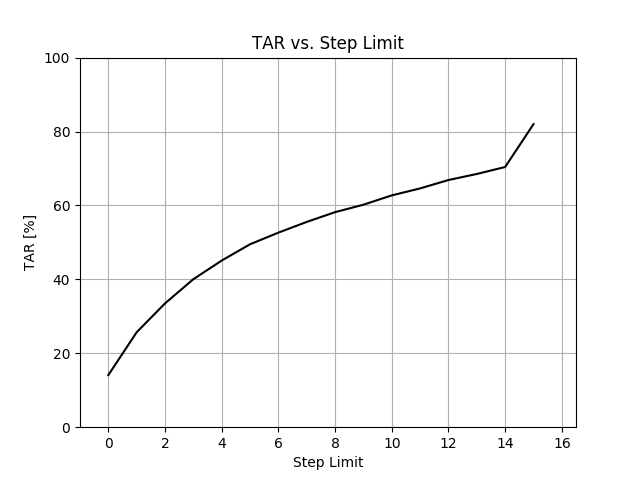
\includegraphics[width=0.5\textwidth]{figures/cdf_tar_limit.png}
  \caption{The distribution of the TAR as a function of the step limit for a search. }\label{fig:tar-steps}
\end{figure}

%\begin{figure}
  %\centering
  %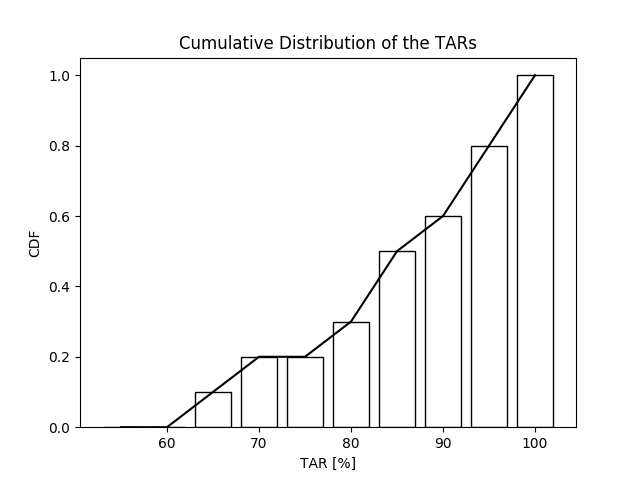
\includegraphics[width=0.5\textwidth]{figures/cdf_tar.png}
  %\caption{A plot giving the cumulative proportion of searches that successfully found the target object before reaching the 16-step limit. }\label{fig:complete-searches-subjects}
%\end{figure}

Table~\ref{tab:results-full} shows a fairly consistent spread for the TAR across the participants. The inter-participant spread ($\sigma=11\%$) is fairly significant, perhaps indicating that the user's search behaviour and strategy affects the target acquisition performance, but with an average TAR of $81.2\%$, it is clear that the system successfully finds the target object during the vast majority of searches. 

Figure~\ref{fig:tar-objects} shows the TAR for each object in $\mathbf{O}$. From it, we can see that there are variations the TAR for the different objects, with the smaller objects typically being the hardest to find. However, the differences are not extreme and indicate that all the objects in $\mathbf{O}$ are roughly equally hard to find. This is also displayed in the simulation's TAR in Table~\ref{tab:results-summary}, which could not achieve 100\% because of the difficulty the agent had in finding the objects on the fringes of the environment. 


\begin{figure}
  \centering
  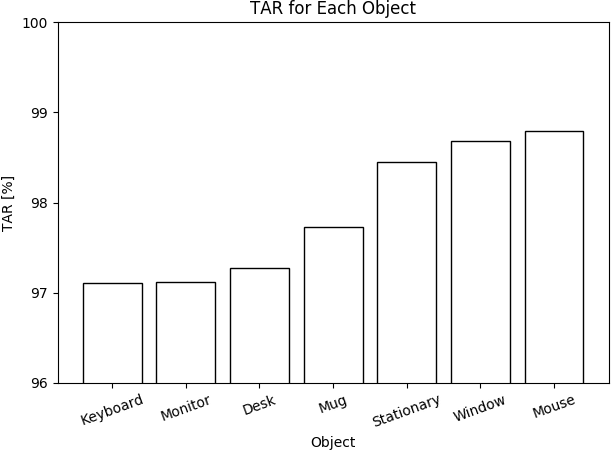
\includegraphics[width=0.45\textwidth]{figures/tar_objects.png}
  \caption{The TAR for each of the objects within the target object set. }\label{fig:tar-objects}
\end{figure}

The TAR can be improved with regards to entering a no-recovery state where it directs a user into dead-space with no spatial information (e.g.\ a ceiling or wall section) and cannot gather the information it requires to intelligently guide the user. Subsequent system updates will have to consider implementing fall-back methods or other automatic recovery modes that can detect entry of a no-recovery state (e.g.\ exceeding a set number of steps/time without making an observation) and guide the user back to the initial position.

\subsubsection{Number of Steps to Target}

\noindent The number of steps target indicates the number of waypoints the system generated for the participant during the guidance process and is a major indication of system performance, where less waypoints means faster target acquisition and better performance. Figure~\ref{fig:nsteps-participants} shows the cumulative distribution of the number of steps to the target for all the participants. 

\begin{figure}
  \centering
  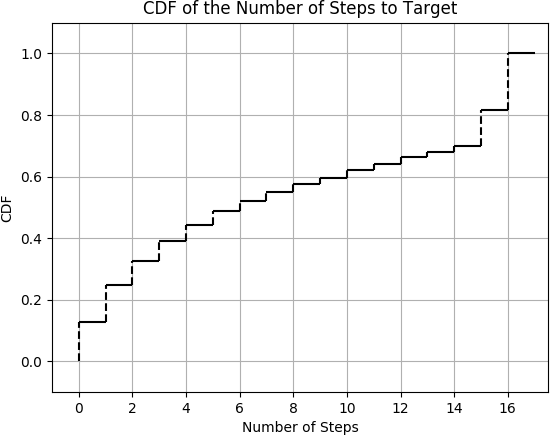
\includegraphics[width=0.5\textwidth]{figures/cdf_total_steps.png}
  \caption{The cumulative distribution of the participants' number of steps taken to find a target object. }\label{fig:nsteps-participants}
\end{figure}

The number of waypoints each participant required is fairly evenly spread across all of the participants. The population mean and standard deviation is 6.8 and 5.1 waypoints respectively. This is a reasonable result that was also somewhat expected, since most target objects were placed within approximately 4 grid squares away from the participants' initial looking directions. However, the relatively high standard deviation should be noted and can also be reduced by implementing the automatic recovery mode mentioned previously, and avoiding information-sparse areas.

As expected, the number of steps on the simulation required on average to find the target object is less than for the experiments. The full set of results for the simulation is given by a frequency mapping of the coincidences between the simulation and experimental data in Figure~\ref{fig:sim-vs-experiment}.

\begin{figure}
  \centering
  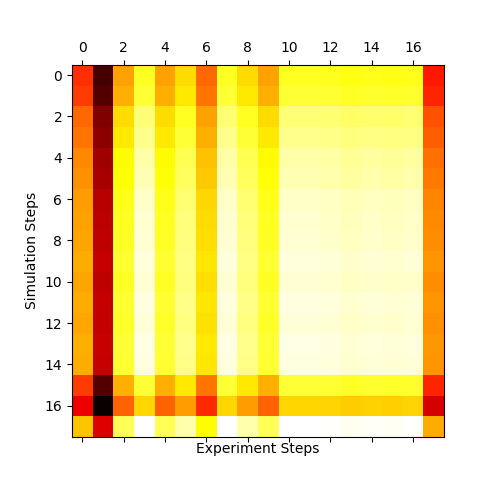
\includegraphics[width=0.5\textwidth]{figures/experiment_vs_simulation.png}
  \caption{A summary of the experiment and simulation steps to target results. }\label{fig:sim-vs-experiment}
\end{figure}

% It is interesting to note that participants $s6$ and $s10$ also found their targets within these reasonable bounds when accounted for the targets that they found within the 16-step limit. This supports the argument from the previous results that their decreased TAR was partly caused by an abnormally high number of entries into a no-recovery state and further reinforces the need to implement an automatic recovery feature in the system before deployment. 

\subsubsection{Time to Target}

\noindent The distribution of the total time it took the participants to reach the target object is given in Figure~\ref{fig:time-participants}. We see that the distribution is heavily skewed to the bottom with a long tail. The mean and standard deviation of the data is 29.8s and 23s respectively. %, is far greater than for the number of waypoints they required. Indeed, there is not a strong relationship between the number of waypoints a participant required and the time they took to find the target, as showcased by participant $s7$'s wide mean waypoint count and spread in Figure~\ref{fig:nsteps-participants} and the small spread and close-to-average time to target in Figure~\ref{fig:time-participants}. Furthermore, the opposite can be observed in participant $s8$'s small spread and low mean waypoint count in Figure~\ref{fig:nsteps-participants} and high spread and high mean time to target in Figure~\ref{fig:time-participants}. 

\begin{figure}
  \centering
  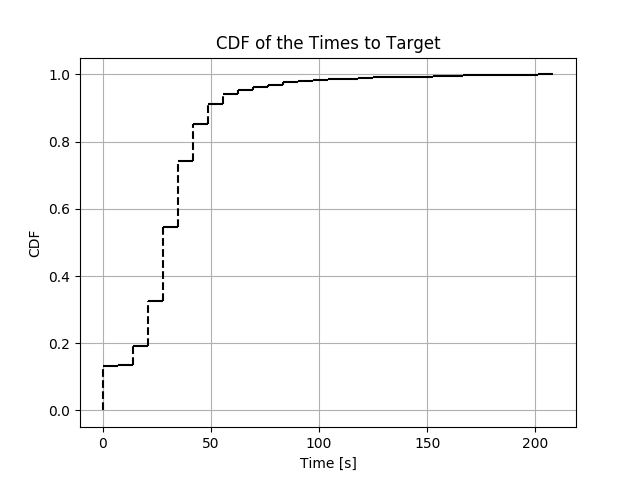
\includegraphics[width=0.5\textwidth]{figures/cdf_total_time.png}
  \caption{The cumulative distribution of the participants' time taken to find a target object. }\label{fig:time-participants}
\end{figure}

In comparison to the VizWiz system~\cite{bigham2010vizwiz} (mean 92s, standard deviation 37.7s), our results look very reasonable. However, these results may greatly change when we test the system with VI participants like they did in~\cite{bigham2010vizwiz}.

\section{\uppercase{Future Work and Conclusion}}\label{sec:conclusion}

\noindent In this work we presented and tested an MDP-based system to guide a visually impaired (VI) person towards a target object with no apriori knowledge of the environment. We implemented the system in an Android app that we tested with a small group of sighted people to determine its viability and effectiveness at guiding a user to manipulating a camera and finding a target object. We found that is works well when compared to alternative systems, with a respectable mean time of target acquisition of 32s. However, the system can be improved by refining the search strategy and implementing an automatic fail-state recovery system that will guide a user back to neutral position if a fail-state is entered (e.g.\ a blank section of wall). 

The next steps to this project will involve using the data recorded here to improve and refine the MDP model that provides the guidance. The model can also be expanded to include more objects and actions. However, an important consideration and expansion to the problem is to change the MDP to an Partially Observable MDP (POMDP) model that will bring the model more in line with reality by acknowledging that the objects are not perfectly observable and humans do not perfectly follow guidance instructions. This adjustment may be very important when we replace the QR code scanner with an object recognition that are typically more prone to making classification errors. Finally, the model can be adapted to use on-line learning techniques in order to further refine its transition model as the guidance system is used.  

\clearpage
\bibliographystyle{apalike}
\bibliography{bib}

\end{document}
